\section{Conclusion and Discussion}

\subsection{Natural angular frequency}

Although by theory amplitude doesn't affect the period, as the amplitude gets
larger, the negative work done by the frictional force isn't negligible.  
Thus, we need to keep the amplitude the same for every test to reduce this
influence factor.

The third measurement of ten periods is obviously smaller than the other three,
which might result from a severely different amplitude.

On the other hand, by measuring 10 times of T, the experimental value of
$\omega_0$ is quite precise (with small deviation).
Still, $u_{10T,r}=0.07\%$, that means our experiment setup works pretty well.

For recommendation, I think introducing a control system for the amplitude in
addition to bare hand can bring more precison.


% NOTE:DONE

\subsection{Damping coefficient}

The damping coefficient is calculated from dividing the decreasing
amplitude and log it.
When calculating the damping coefficient, successive difference method is applied
to reduce the deviation. 

For more precison than successive difference method, we could use curve fitting,
thus the whole list can be used to determine the damping coefficient $\beta$
from $\theta_n=\theta_0e^{-\beta (nT)}$, instead of only using 5 groups of
isolated points. 

\begin{figure}[H]
\centering
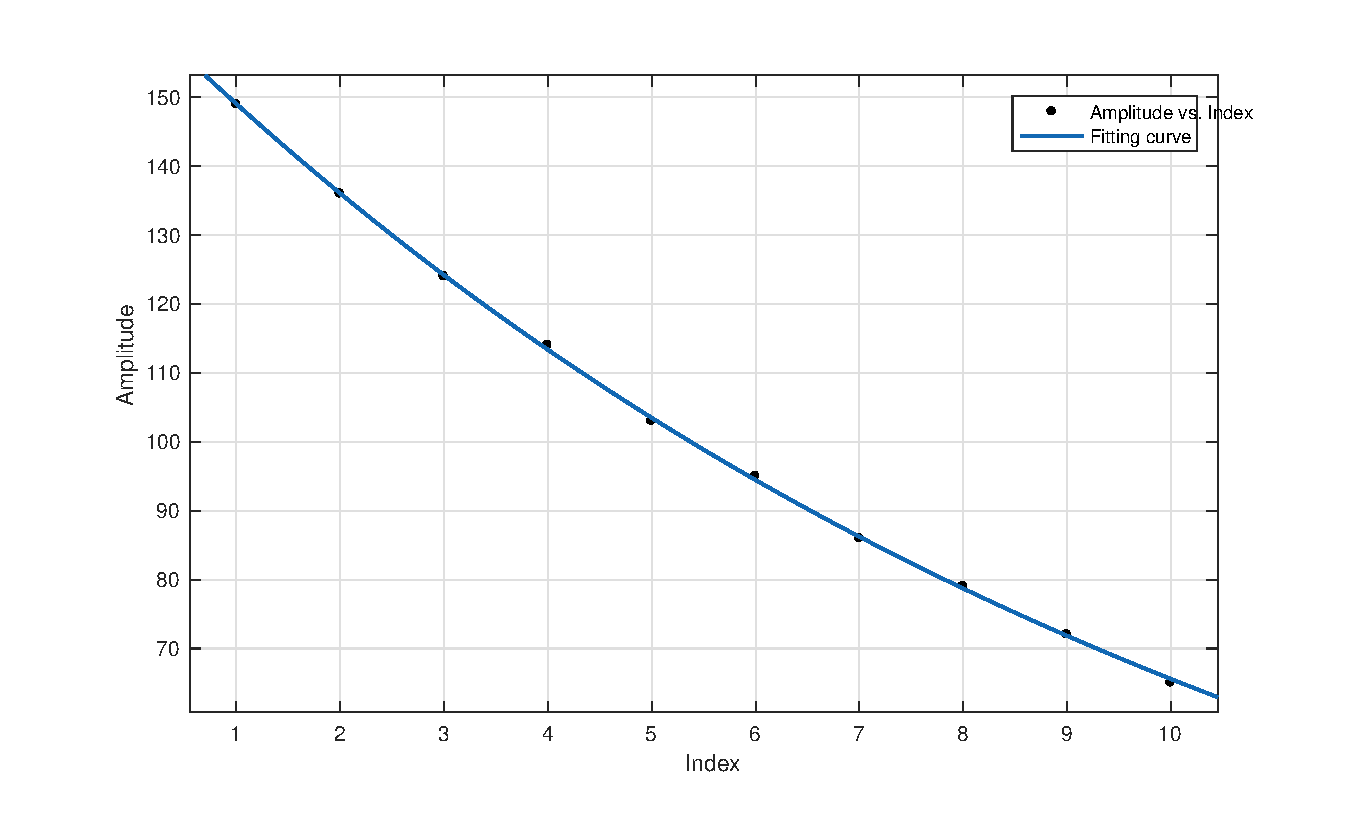
\includegraphics[width=1\textwidth]{matlab/p3}
\caption{Curve fitting example}
\end{figure}

And we can find the b of the curve, which is $-0.09125$
Comparing $- 5\times b =  0.4562 $ with $\beta = 0.4558$
$$ u_{\beta,r}=  0.0878 \% $$

We can reach a conclusion that although curve fitting can introduce more precise
process, the present methode is quite accurate.

% NOTE: Delete a figure

\subsection{$\varphi$ vs. $\omega$}

\subsubsection{Discussions}

Both of the $\varphi$ vs. $\omega$ curve are decreasing in the shape of arc
cotangent (see Figure \ref{phi}). In theory we know that for the smaller damping
coefficient, the left side curve of $\omega/\omega_0=1.0$ is higher than the
other and the right side curve is lower than that. However, our results show
that although the right half of the damping selection 3 curve is higher than
damping selection 2 near the $\omega/\omega_0=1.0$, its gets lower quickly and
beneath the damping selection 2, which is abnormal. We recall the measurement
procedure and conclude that it's blamed on the backslash error. During the
second half of the experiment we thought the $\omega$ gap we chose is too small
so we relatively quickly rotated the knob but made the gap too big. Therefore,
we rotated the knob inversely to measure the middle $\omega$ again. Also, the
time duration will be longer to reach the stable situation. This causes the
second half of phase shifts to be smaller. 

\subsubsection{Improvements and recommendations}

During the experiment we find it hard to predict the phase shift. We can only
see the strobe flashes and read the phase shift. There are two methods to this
problem. 

\begin{enumerate}
\item Rotate the knob very carefully and be patient enough to read the phase
  shift for more times until it's stable. Patience can eliminate the deviation. 
\item Redesign the machine. If there's an easier way to directly change the
  phase shift to the expected value, the entire experiment will be easy. 
\end{enumerate}

Whichever improvement we make, we have to be patient to ensure the oscillation
is stable. 

\subsection{$\theta_{st}$ vs. $\omega$}

\subsubsection{Discussions}

The shape of both curve are within our expectation (see Figure~\ref{theta}).
Obviously, the damping coeffiecient 2 is smaller than damping coeffiecient 3
beacuse the entire curve of damping selection 2 is above the curve of damping
selection 3. we find that their beginning are roughly the same. However, it's
hard to tell whether the peaks occur on the left or right hand side of the
straight line $\omega/\omega_0=1.0$. In our expectation, the peaks should occur
on the slightly left of the straight line. We suppose it's because the
oscillation has not been stable yet. The value of $10T$ is smaller so that the
calculated $\omega$ is larger than the real value, which makes the entire curve
move rightwards. Therefore, the peak does not occur on the slightly left of
$\omega/\omega_0=1.0$. 


% NOTE: Finish below
\subsubsection{Improvements and recommendations}

It hurts for us to bear the flashlight for reading the phase data. Electronic
devices such as a camera can be introduced to record the data, instead of
directly reading the data with human eyes.